\section{Classic CPU Vulnerabilities}
\frame{\sectionpage}

\begin{frame}{Spectre}{Discovered by Paul Kocher (Independent) and Jann Horn (Google Project Zero)}
    \label{spectre}
    \begin{columns}
        \begin{column}{0.5\textwidth}
            \begin{itemize}
                \item \href{https://spectreattack.com/spectre.pdf}{\color{pink}Spectre} relies on mistraining the CPU branch predictor, which can happen when an attacker can execute machine code or even remotely via rop-style gadgets.
                \item When a misprediction occurs, the processor should revert to a "snapshot" state before the bad branch.
                \item However, caches are not reverted, thus an attacker can leak data going into the cache from speculation!
            \end{itemize}
            \usemintedstyle{vim}
            \inputminted{c}{code/spectre.c}
        \end{column}
        \begin{column}{0.5\textwidth}
            \begin{figure}
                \centering
                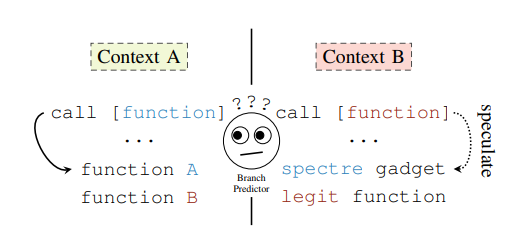
\includegraphics[width=\textwidth]{images/spectre_paper_graphic.png}
                \caption{An attacker controlled Context A mistrains the branch predictor in the victim context B.}
                \label{fig:spectre-graphic}
            \end{figure}
        \end{column}
    \end{columns}
    \note{
        \begin{itemize}
            \item Spectre gained notoriety because it can be exploited \textit{remotely}, unlike previous CPU attacks which required local execution.
            \item Data is leaked from an arbitrary context since the branch predicate confuses data and code during speculation. 
            \item For a more modern branch predictor attack, see Ghostrace.
        \end{itemize}
    }
\end{frame}

\begin{frame}{Prime+Probe}{Dag Arne Osvik et al. of Weizmann Institute of Science}
    \label{prime+probe}
    \href{https://cs-people.bu.edu/tromer/papers/cache.pdf}{\color{pink}Prime+Probe} is a very old technique primarily shown to break data-dependent access cryptographic implementations (i.e. table-based). 
    \begin{enumerate}
        \item An attacker first \textit{primes} the data cache by accessing every line within the cache. 
        \item Then, the victim process runs some sensitive algorithm, say AES.
        \item The attacker then measures their own memory accesses to determine which memory was accessed.
    \end{enumerate}
    Notably, this attack requires knowledge of the algorithm! Many side-channeling attacks require knowledge of the algorithm, affecting exploitability. 
    \note{
        \begin{itemize}
            \item In AES S-Boxes, lookups are linear-ish. So depending on which part of the giant array was accessed, gleans information to the attacker.
            \item This attack targeted L1 caches, it was eventually expanded on by other researchers to target last-level caches.
            \item A key component to this attack was knowledge of how memory addresses translated into cache lines; this is called a microarchitectural hash function, and nowadays this function is very complex!
        \end{itemize}
    }
\end{frame}

